\documentclass[a4paper,11pt]{article}
%BIBLIOTECAS==================================================================================%
\usepackage[latin1]{inputenc}
\usepackage[brazil]{babel}
\usepackage{fancyhdr}
\usepackage{amsmath}
\usepackage{amsfonts}
\usepackage{amssymb}
\usepackage{graphicx} %para inserir figuras
\usepackage{subfigure} %para inserir subfiguras
\usepackage{url} %para links
\usepackage[normalem]{ulem}
\usepackage{titlesec}
\usepackage{setspace}
\usepackage{cite}
\usepackage{indentfirst} %primeiro par�grafo
\usepackage[font=small,format=plain,labelfont=bf,up,up]{caption} %customiza legendas
\usepackage[a4paper,left=3cm,bottom=2cm,right=2cm,top=3cm]{geometry} %para definir as margens
\usepackage{listings} %para formatar c�digo-fonte
\lstset{numbers=left, numberstyle=\tiny, stepnumber=1, numbersep=5pt,basicstyle=\scriptsize,frame=single} %para c�digos
\usepackage{float} %posicao das legendas
\usepackage{multicol} %subcolunas
\usepackage{multirow}
\usepackage{enumitem} %itens
%=============================================================================================%
\setlength{\parindent}{25pt}
\setlength{\parskip}{0ex}
\onehalfspacing
%=============================================================================================%
%\titleformat{\part}[frame]{\normalfont}{\filright\footnotesize\enspace\thepart\enspace}{1em}{\Large\bfseries\filcenter}
%\titleformat{\section}[block]{\bfseries}{\thesection.}{1em}{\MakeUppercase}
%\titleformat{\subsection}[block]{\normalfont}{\thesubsection.}{1em}{\MakeUppercase}
%\titleformat{\subsubsection}[block]{\normalfont}{\thesubsubsection.}{1em}{}
\renewcommand{\lstlistingname}{Script}
\DeclareCaptionLabelSeparator{minus}{ - }
\captionsetup[FLOAT_TYPE]{labelformat=simple, labelsep=colon}
\captionsetup[figure]{labelsep=minus}
\captionsetup[table]{labelsep=minus}
\captionsetup[lstlisting]{labelsep=minus}
\floatstyle{plaintop}\restylefloat{table} %legenda das tabelas no topo
\addtolength{\belowcaptionskip}{-4pt} %espaco entre legendas
\addtolength{\abovecaptionskip}{-2pt}

%=============================================================================================%
\begin{document}
	\thispagestyle{empty}

\begin{figure}[t]
\centering

\includegraphics[scale=0.6]{imagens/Logo.png}
\end{figure}

{\centering\linethickness{3pt}\line(1,0){455}}\\

\begin{large}
	\centering
	CENTRO DE TECNOLOGIA E URBANISMO\\
	DEPARTAMENTO DE ENGENHARIA EL�TRICA\\
	2ELE047 - Gera��o, Transmiss�o e Distribui��o\\[1.4in]
	\textbf{Fluxo de Pot�ncia}\\[.2in]
	\begin{tabular}{rl}
	PROFESSOR:& Luis Alfonso Gallego Pareja\\
	ALUNOS:   & Ricardo Tadashi Kobayashi
	\end{tabular}
	\\[1.1in]
\end{large}

\begin{flushright}
\parbox{2.1in}
{
Relat�rio apresentado a disciplina de Gera��o, Transmiss�o e Distribui��o.\\

Turma: 1000.\\[1.2in]
}
\end{flushright}

\begin{large}
	\begin{center}
	
	Londrina, \today \\
	\end{center}
\end{large}

{\centering\linethickness{3pt}\line(1,0){455}}
	\thispagestyle{empty} 
\tableofcontents 
\pagebreak 
%\thispagestyle{empty} 
%\listoffigures 
%\listoftables 
%\pagebreak
	%\section{RESUMO}

Um sistema de comunica��es digitais PAM retangular que utilize di-bit 00, 01, 10, e 11 para representar os s�mbolos respectivamente, caso for mal interpretado na recep��o dos valores intermedi�rios causa o erro de dois bits de sinal. Com a utiliza��o do c�digo Gray (00, 01, 11 e 10) a interpreta��o de um s�mbolo adjacente produz o erro de somente um bit. 
\vspace{9pt}

\noindent \textit{Palavras-chave: C�digo Gray, performance, canal AWGN, Modula��o PAM}

	\section{OBJETIVOS}
Este trabalho ir� expor os resultados da resolu��o de um problema de fluxo de pot�ncia composto por 14 barras, os quais foram obtidos atrav�s de algor�timos desenvolvidos no Matlab. Neste caso, foram desenvolvidos cinco algor�timos para a resolu��o de tal problema: o m�todo de Newton, o m�todo de Newton desacoplado 1, o m�todo de Newton desacoplado 2, o m�todo desacoplado r�pido e o m�todo DC. Al�m de se resolver o problema, ser� feita uma compara��o entre os algor�timos, em termos de precis�o e complexidade computacional.


	\section{TEORIA}
Esta se��o apresentar� os conceitos empregados na execu��o da atividade relatada.


\subsection{Descri��o do problema}
A figura abaixo representa o sistema el�trico de pot�ncia:
\begin{figure}[H]
	\centering
	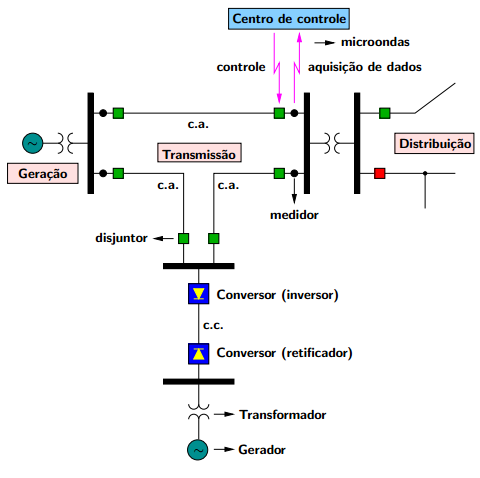
\includegraphics[scale=.7]{imagens/modelo}
	\caption{Gera��o, transmiss�o e distribui��o}
\end{figure}

O estudo do fluxo de pot�ncia na transmiss�o permite definir as condi��es de opera��o dos elementos e fluxo de carga entre linhas. Para isso, a transmiss�o � representada atrav�s de barras, nas quais s�o ligadas cargas, geradores e outros elementos, e linhas, que ligam duas barras distintas. Neste estudo, admite-se um n�mero n de barras, o que dificulta a an�lise, exigindo uma modelagem mais gen�rica.

\subsubsection{Tipos de Barras}
Neste estudo ser�o classificadas tr�s tipos de barras:
\begin{table}[H]
	\centering
	\footnotesize
	\begin{tabular}{c|c|c}\hline
		\textbf{Tipo} & \textbf{Vari�veis conhecidas} & \textbf{Vari�veis desconhecidas}    \\\hline
		$PQ$          & $P,Q$						  & $V,\theta$							\\\hline
		$PV$          & $P,V$						  & $Q,\theta$								\\\hline
		$V\theta$     & $V,\theta$					  & $P,Q$								\\\hline
	\end{tabular}
	\caption{Tipos de barras}
\end{table}

\subsubsection{Modelo da linha}
No geral, as an�lises do fluxo de pot�ncia usam o modelo $\pi$. Tal modelo contempla as resist�ncias, indut�ncias e capacit�ncias presentes entre duas linhas:
\begin{figure}[H]
	\centering
	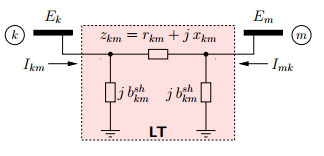
\includegraphics[scale=.8]{imagens/pi}
	\caption{Modelo $\pi$ da linha}
\end{figure}

Onde:
\begin{multicols}{2}
\begin{itemize}[noitemsep,nolistsep]
	\item $r_{km}$: resist�ncia s�rie;
	\item $x_{km}$: reat�ncia indutiva s�rie;
	\item $b_{k}^{sh}$: suscept�ncia shunt;
	\item $z_{km}$: imped�ncia s�rie;
	\item $y_{km}=1/z_{km}$: admit�ncia s�rie;
	\item $g_{km}=Re(y_{km})$: condut�ncia s�rie;
	\item $b_{km}=Im(y_{km})$: suscept�ncia s�rie.
\end{itemize}
\end{multicols}


Neste modelo, a admit�ncia nodal � dada por:
\begin{equation}
	\begin{cases}
		\begin{array}{rcl}
			Y_{km} & = & -y_{km}\\
			Y_{mk} & = & -y_{km} \\
			Y_{mk} & = & j\cdot b_k^{sh} + \displaystyle\sum\limits_{k\in\Omega_k}^{} j\cdot b_k^{sh} + y_{km}
		\end{array}
	\end{cases}
\end{equation}

Al�m disso, a condut�ncias e a suscept�ncias nodais ficam:
 \begin{equation}
	\begin{cases}
		\begin{array}{rcl}
			G_{km} & = & Re(Y_{km})\\
			B_{km} & = & Im(Y_{km})
		\end{array}
	\end{cases}
\end{equation}

\subsubsection{Pot�ncias e perdas}
As pot�ncias, ativas e reativas nodais s�o dadas respectivamente por:
\begin{equation}
	\begin{cases}
		\begin{array}{rcl}
			P_{k} & = & V_k \cdot \displaystyle\sum\limits_{k\in\Omega_k}^{} V_m\cdot (G_{km}\cdot cos\theta_{km}+B_{km}\cdot sen\theta_{km})\\
			Q_{k} & = & V_k \cdot \displaystyle\sum\limits_{k\in\Omega_k}^{} V_m\cdot (G_{km}\cdot cos\theta_{km}-B_{km}\cdot sen\theta_{km})\\
		\end{array}
	\end{cases}
\end{equation}

J� as pot�ncias entre duas barras podem ser computadas por:
\begin{equation}
	\begin{cases}
		\begin{array}{rcl}
			P_{km} & = & g_{km}\cdot V_{k}^2 - V_{k}\cdot V_{m} \cdot ( g_{km}\cdot cos\theta_{km} + b_{km}\cdot sen\theta_{km} )\\
			Q_{km} & = & -(b_{km}+b_{km}^{sh})\cdot V_{k}^2 - V_{k}\cdot V_{m} \cdot ( g_{km}\cdot sen\theta_{km} - b_{km}\cdot cos\theta_{km} )\\
			P_{mk} & = & g_{km}\cdot V_{m}^2 - V_{k}\cdot V_{m} \cdot ( g_{km}\cdot cos\theta_{km} - b_{km}\cdot sen\theta_{km} )\\
			Q_{mk} & = & -(b_{km}+b_{km}^{sh})\cdot V_{m}^2 + V_{k}\cdot V_{m} \cdot ( g_{km}\cdot sen\theta_{km} + b_{km}\cdot cos\theta_{km} )\\
		\end{array}
	\end{cases}
\end{equation}

Por fim as perdas nas linhas s�o dadas por:
\begin{equation}
	\begin{cases}
		\begin{array}{rcl}
			Pperdas_{km} & = & P_{km}+P_{mk}\\
			Qperdas_{km} & = & Q_{km}+Q_{mk}\\
		\end{array}
	\end{cases}
\end{equation}

\subsection{M�todo de Newton}
No m�todo de Newton o problema proposto � resolvido da forma completa de forma num�rica utilizando o m�todo de Newton, atrav�s da matriz jacobiana:
\begin{equation}
	\left[
		\begin{array}{c}
			\mathbf{\Delta P}\\
			\mathbf{\Delta Q}		
		\end{array}
	\right]^{(i)}
	=
	\left[
		\begin{array}{cc}
			\mathbf{H} & \mathbf{N}\\
			\mathbf{M} & \mathbf{L}
		\end{array}
	\right]^{(i)}
	\cdot
	\left[
		\begin{array}{c}
			\mathbf{\Delta \theta}\\
			\mathbf{\Delta V}		
		\end{array}
	\right]^{(i)}
\end{equation}

O sistema descrito anteriormente � calculada para as barras do tipo $PQ$ e $PV$.

Considera-se para resolu��o do problema a diferen�a entre as pot�ncias estimadas e as pot�ncias calculadas ao longo do processo, a qual tamb�m � utilizada como um crit�rio de converg�ncia:
\begin{equation}
	\begin{array}{rcl}
		\mathbf{\Delta P} & = & \mathbf{P_{est}} - \mathbf{P}\\
		\mathbf{\Delta Q} & = & \mathbf{Q_{est}} - \mathbf{Q}
	\end{array}
\end{equation}

No caso das tens�es e �ngulos, tem-se:
\begin{equation}
	\begin{array}{rcl}
		\mathbf{\Delta P}      & = & \mathbf{V^{(i+1)}} - \mathbf{P^{(i)}}\\
		\mathbf{\Delta \theta} & = & \mathbf{\theta^{(i+1)}} - \mathbf{Q^{(i)}}
	\end{array}
\end{equation}

Onde o �ndice $(i)$ representa a itera��o do processo.

Os elementos que relacionam as tens�es e �ngulos com as pot�ncias s�o descritos abaixo:
\begin{equation}
	\begin{cases}
		\begin{array}{rcl}
			H_{kk} & = & -B_{kk} \cdot V_{k}^2 - Q_{k}\\
			H_{km} & = & +V_{k}\cdot V_{m} \cdot ( G_{km}\cdot sen\theta_{km} - B_{km}\cdot cos\theta_{km} ) \\
			H_{mk} & = & -V_{k}\cdot V_{m} \cdot ( G_{km}\cdot sen\theta_{km} + B_{km}\cdot cos\theta_{km} ) 
		\end{array}
	\end{cases}
\end{equation}

\begin{equation}
	\begin{cases}
		\begin{array}{rcl}
			N_{kk} & = & -V_{k}^{-1} \cdot ( P_{k} + G_{kk}\cdot V_{k}^2 )\\
			N_{km} & = & +V_{k} \cdot ( G_{km}\cdot cos\theta_{km} + B_{km}\cdot sen\theta_{km} ) \\
			N_{mk} & = & -V_{m} \cdot ( G_{km}\cdot cos\theta_{km} - B_{km}\cdot sen\theta_{km} ) 
		\end{array}
	\end{cases}
\end{equation}

\begin{equation}
	\begin{cases}
		\begin{array}{rcl}
			M_{kk} & = & -G_{kk} \cdot V_{k}^2 + P_{k}\\
			M_{km} & = & -V_{k}\cdot V_{m}\cdot ( G_{km}\cdot cos\theta_{km} + B_{km}\cdot sen\theta_{km} ) \\
			M_{mk} & = & -V_{m}\cdot V_{k}\cdot ( G_{km}\cdot cos\theta_{km} - B_{km}\cdot sen\theta_{km} ) 
		\end{array}
	\end{cases}
\end{equation}

\begin{equation}
	\begin{cases}
		\begin{array}{rcl}
			L_{kk} & = & V_{k}^{-1} \cdot ( Q_k - B_{kk}\cdot V_{k}^2 )\\
			L_{km} & = & +V_{k} \cdot ( G_{km}\cdot sen\theta_{km} - B_{km}\cdot cos\theta_{km} ) \\
			L_{mk} & = & -V_{m} \cdot ( G_{km}\cdot sen\theta_{km} + B_{km}\cdot cos\theta_{km} ) 
		\end{array}
	\end{cases}
\end{equation}

Ap�s realizar uma itera��o as as tens�es e os �ngulos devem ser atualizados e � feito um teste de converg�ncia. Caso o resultado ainda n�o convirja, o Jacobiano deve ser calculado novamente para passar para a pr�xima itera��o. 

O processo iterativo continua at� que se obtenha um erro m�nimo estipulado por:
\begin{equation}
	\begin{array}{rcl}
		erro & > & max([\mathbf{\Delta P} \quad \mathbf{\Delta Q}])
	\end{array}
\end{equation}


Feito isso, o subsistema 2 � resolvido. Este consiste basicamente em calcular as pot�ncias reativas para as barras $PV$ e as pot�ncias ativas e reativas para as barras $V\theta$.











\subsection{M�todo desacoplado 1}
O m�todo desacoplado 1 tem baseia-se no m�todo de Newton, mas neste caso despreza-se as matrizes $\mathbf{M}$ e $\mathbf{N}$, sendo poss�vel achar os �ngulos e as tens�es das barras de forma independente.
\begin{equation}
	\left[
		\begin{array}{c}
			\mathbf{\Delta P}^{(p)}\\
			\mathbf{\Delta Q}^{(q)}		
		\end{array}
	\right]
	=
	\left[
		\begin{array}{cc}
			\mathbf{H}^{(p)} & \mathbf{0}\\
			\mathbf{0} & \mathbf{L}^{(q)}
		\end{array}
	\right]
	\cdot
	\left[
		\begin{array}{c}
			\mathbf{\Delta \theta}^{(p)}\\
			\mathbf{\Delta V}^{(q)}		
		\end{array}
	\right]
\end{equation}

No caso deste m�todo, as matrizes $\mathbf{H}$ e $\mathbf{L}$ s�o as mesmas do m�todo de Newton, logo elas podem ser consultadas na se��o anterior.

Como os m�todos desacoplados permitem a solu��o das vari�veis $\mathbf{V}$ e $\mathbf{\theta}$ de forma independente, o crit�rio de teste da converg�ncia � feito de maneira diferente. Os m�todos desacoplados seguem o seguinte algor�timo para a solu��o do problema:
\begin{figure}[H]
	\centering
	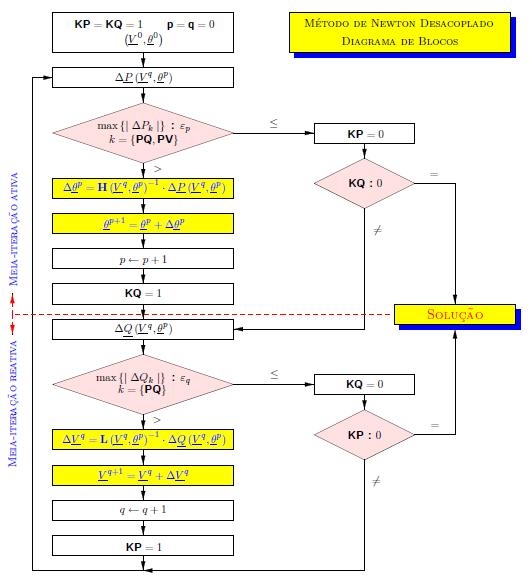
\includegraphics[scale=0.7]{imagens/fluxograma}
	\caption{Fluxograma para o algor�timo aplicado aos m�todos desacoplados}
\end{figure}
 
Desta forma, os problemas ativo e reativo podem apresentar velocidades diferentes de converg�ncia. Por isso, as itera��es s�o contadas separadamente pelos contadores p e q.


\subsection{M�todo desacoplado 2}
O m�todo desacoplado pode ser alterado dividindo o fluxo l�quido de pot�ncia pelas tens�es:
\begin{equation}
	\left[
		\begin{array}{c}
			\mathbf{\Delta P/V}^{(p)}\\
			\mathbf{\Delta Q/V}^{(q)}	
		\end{array}
	\right]
	=
	\left[
		\begin{array}{cc}
			\mathbf{H'}^{(p)} & \mathbf{0}\\
			\mathbf{0} & \mathbf{L'}^{(q)}
		\end{array}
	\right]
	\cdot
	\left[
		\begin{array}{c}
			\mathbf{\Delta \theta}^{(p)}\\
			\mathbf{\Delta V}^{(q)}		
		\end{array}
	\right]
\end{equation}

Desta forma a matriz de desacoplamento � alterada:
\begin{equation}
	\begin{cases}
		\begin{array}{rcl}
			H_{kk}' & = & -B_{kk} \cdot V_{k} - Q_{k}/V_{k}\\
			H_{km}' & = & +V_{m} \cdot ( G_{km}\cdot sen\theta_{km} - B_{km}\cdot cos\theta_{km} ) \\
		\end{array}
	\end{cases}
\end{equation}


\begin{equation}
	\begin{cases}
		\begin{array}{rcl}
			L_{kk}' & = & Q_k / V_{k} - B_{kk} \cdot V_{k} \\
			L_{km}' & = & +V_{m} \cdot ( G_{km}\cdot sen\theta_{km} - B_{km}\cdot cos\theta_{km} ) \\
		\end{array}
	\end{cases}
\end{equation}



















\subsection{M�todo desacoplado r�pido}
Neste m�todo, considera-se mais aproxima��es, as quais exigem algumas condi��es a serem satisfeitas:
\begin{itemize}[noitemsep,nolistsep]
	\item Sistema pouco carregado, o que faz com que $\theta_{km}$ seja pequeno e que $cos\theta_{km}$ seja aproximadamente unit�rio;
	\item Tens�es pr�ximas a 1 pu;
	\item Rela��o $B_{km}/G_{km}$ alta.
\end{itemize}

O sistema a ser resolvido se torna:
\begin{equation}
	\left[
		\begin{array}{c}
			\mathbf{\Delta Q/V}^{(q)}\\
			\mathbf{\Delta P/V}^{(p)}	
		\end{array}
	\right]
	=
	\left[
		\begin{array}{cc}
			\mathbf{B'} & \mathbf{0}\\
			\mathbf{0} & \mathbf{B''}
		\end{array}
	\right]
	\cdot
	\left[
		\begin{array}{c}
			\mathbf{\Delta \theta}^{(q)}\\
			\mathbf{\Delta V}^{(p)}		
		\end{array}
	\right]
\end{equation}

Respeitadas as exig�ncias e desprezando a resist�ncia para o c�lculo dos elementos $\mathbf{B'}$, os par�metros do sistemas assumem as caracter�sticas mostradas abaixo. Esta aproxima��o, no m�todo desacoplado r�pido � conhecida como m�todo XB, e possui a melhor velocidade de converg�ncia na grande maioria dos casos. 
\begin{equation}
	\begin{cases}
		\begin{array}{rcl}
			B'_{kk} & = & \displaystyle\sum\limits_{k\in\Omega_k}^{} \dfrac{1}{x_{km}}\\
			B'_{km} & = & -\dfrac{1}{x_{km}} 
		\end{array}
	\end{cases}
\end{equation}
\begin{equation}
	\begin{cases}
		\begin{array}{rcl}
			B''_{kk} & = & -B_{kk}\\
			B''_{km} & = & -B_{km} \\
		\end{array}
	\end{cases}
\end{equation}

Nota-se que os valores de $\mathbf{B'}$ e $\mathbf{B''}$ n�o mudam ao longo do processo iterativo, o que torna o m�todo menos complexos.















\subsection{M�todo DC}
O m�todo DC � baseado no acoplamento $P\theta$, logo ele s� leva em conta o fluxo ativo de pot�ncia. Neste m�todo, s�o feitas mais aproxima��es do que no m�todo desacoplado r�pido:
\begin{itemize}[noitemsep,nolistsep]
	\item �ngulos das tens�es muito pequenos, ou seja $sen\theta_{km}\approx \theta_{km}$;
	\item Tens�es unit�rias em todas as barras 1 pu;
	\item Resist�ncia s�rie da linha nula, $r_{km} = 0$.
\end{itemize}

Dadas essas aproxima��es, o problema se resume a:
\begin{equation}
	\mathbf{\Delta P} = \mathbf{B'} \cdot \mathbf{\Delta\theta}
\end{equation}

Onde:
\begin{equation}
	\begin{cases}
		\begin{array}{rcl}
			B'_{kk} & = & \displaystyle\sum\limits_{k\in\Omega_k}^{} \dfrac{1}{x_{km}}\\
			B'_{km} & = & -\dfrac{1}{x_{km}} 
		\end{array}
	\end{cases}
\end{equation}
	\section{METODOLOGIA EXPERIMENTAL}
Como dito anteriormente, esta atividade teve como objetivo o desenvolvimento de algor�timos capaz de resolver o problema de fluxo de carga. Para test�-los, foi utilizado um problema composto por 14 barras.

As barras do sistema em quest�o possuem as caracter�sticas apresentadas abaixo. As barras est�o enumeradas e classificadas quanto ao seu tipo, sendo o tipo 0 barras PQ, o tipo 2 barras PV e tipo 3 barras $V\theta$. As barras que n�o possuem tens�o controladas tomar�o valores unit�rios (em pu) e os �ngulos das tens�o ser�o considerados nulos. Al�m disso, as pot�ncias ser�o transformadas em pu, sendo a unidade base $100\,[kVA]$
\begin{table}[H]
	\centering
	\scriptsize
	\begin{tabular}{c|c|c|c|c|c|c}\hline
	\multirow{2}{*}{\textbf{Barra}}   & \multirow{2}{*}{\textbf{Tipo}} & \textbf{Tens�o} & \multicolumn{2}{ |c| }{\textbf{Pot�ncia Gerada [kVA]}} & \multicolumn{2}{ |c }{\textbf{Pot�ncia demandada [kVA]}} \\\cline{4-7}
     & & \textbf{Controlada [pu]} & \textbf{Ativa} & \textbf{Reativa} & \textbf{Ativa} & \textbf{Reativa}\\\hline
	%\textbf{Barra} & \textbf{Tipo} & \textbf{Tens�o} & \textbf{Pot�ncia gerada}
	$1$ & $3$ & $1.060E+00$ & $2.324E+02$ & $-1.690E+01$ & $0.000E+00$ & $0.000E+00$   \\\hline
	$2$ & $2$ & $1.045E+00$ & $4.000E+01$ & $4.240E+01$ & $2.170E+01$ & $1.270E+01$   \\\hline
	$3$ & $2$ & $1.010E+00$ & $0.000E+00$ & $2.340E+01$ & $9.420E+01$ & $1.900E+01$   \\\hline
	$4$ & $0$ & $0.000E+00$ & $0.000E+00$ & $0.000E+00$ & $4.780E+01$ & $-3.900E+00$   \\\hline
	$5$ & $0$ & $0.000E+00$ & $0.000E+00$ & $0.000E+00$ & $7.600E+00$ & $1.600E+00$   \\\hline
	$6$ & $2$ & $1.070E+00$ & $0.000E+00$ & $1.220E+01$ & $1.120E+01$ & $7.500E+00$   \\\hline
	$7$ & $0$ & $0.000E+00$ & $0.000E+00$ & $0.000E+00$ & $0.000E+00$ & $0.000E+00$   \\\hline
	$8$ & $2$ & $1.090E+00$ & $0.000E+00$ & $1.740E+01$ & $0.000E+00$ & $0.000E+00$   \\\hline
	$9$ & $0$ & $0.000E+00$ & $0.000E+00$ & $0.000E+00$ & $2.950E+01$ & $1.660E+01$   \\\hline
	$10$ & $0$ & $0.000E+00$ & $0.000E+00$ & $0.000E+00$ & $9.000E+00$ & $5.800E+00$   \\\hline
	$11$ & $0$ & $0.000E+00$ & $0.000E+00$ & $0.000E+00$ & $3.500E+00$ & $1.800E+00$   \\\hline
	$12$ & $0$ & $0.000E+00$ & $0.000E+00$ & $0.000E+00$ & $6.100E+00$ & $1.600E+00$   \\\hline
	$13$ & $0$ & $0.000E+00$ & $0.000E+00$ & $0.000E+00$ & $1.350E+01$ & $5.800E+00$   \\\hline
	$14$ & $0$ & $0.000E+00$ & $0.000E+00$ & $0.000E+00$ & $1.490E+01$ & $5.000E+00$   \\\hline
	\end{tabular}
	\caption{Caracter�sticas das barras}
\end{table}


Os par�metros da linha, j� expressos em pu, s�o mostrados na tabela subsequente:
\begin{table}[H]
	\centering
	\scriptsize
	\begin{tabular}{c|c|c|c|c}\hline
	\textbf{De} & \textbf{Para} & $\mathbf{r_{ij}}$ & $\mathbf{x_{ij}}$ & $\mathbf{Bsh_{ij}}$\\\hline
	$1$  & $2$  & $1.938E-02$ & $5.917E-02$ & $5.280E-02$   \\\hline
	$1$  & $5$  & $5.403E-02$ & $2.230E-01$ & $4.920E-02$   \\\hline
	$2$  & $3$  & $4.699E-02$ & $1.980E-01$ & $4.380E-02$   \\\hline
	$2$  & $4$  & $5.811E-02$ & $1.763E-01$ & $3.400E-02$   \\\hline
	$2$  & $5$  & $5.695E-02$ & $1.739E-01$ & $3.460E-02$   \\\hline
	$3$  & $4$  & $6.701E-02$ & $1.710E-01$ & $1.280E-02$   \\\hline
	$4$  & $5$  & $1.335E-02$ & $4.211E-02$ & $0.000E+00$   \\\hline
	$4$  & $7$  & $0.000E+00$ & $2.091E-01$ & $0.000E+00$   \\\hline
	$4$  & $9$  & $0.000E+00$ & $5.562E-01$ & $0.000E+00$   \\\hline
	$5$  & $6$  & $0.000E+00$ & $2.520E-01$ & $0.000E+00$   \\\hline
	$6$  & $11$ & $9.498E-02$ & $1.989E-01$ & $0.000E+00$   \\\hline
	$6$  & $12$ & $1.229E-01$ & $2.558E-01$ & $0.000E+00$   \\\hline
	$6$  & $13$ & $6.615E-02$ & $1.303E-01$ & $0.000E+00$   \\\hline
	$7$  & $8$  & $0.000E+00$ & $1.762E-01$ & $0.000E+00$   \\\hline
	$7$  & $9$  & $0.000E+00$ & $1.100E-01$ & $0.000E+00$   \\\hline
	$9$  & $10$ & $3.181E-02$ & $8.450E-02$ & $0.000E+00$   \\\hline
	$9$  & $14$ & $1.271E-01$ & $2.704E-01$ & $0.000E+00$   \\\hline
	$10$ & $11$ & $8.205E-02$ & $1.921E-01$ & $0.000E+00$   \\\hline
	$12$ & $13$ & $2.209E-01$ & $1.999E-01$ & $0.000E+00$   \\\hline
	$13$ & $14$ & $1.709E-01$ & $3.480E-01$ & $0.000E+00$   \\\hline
	\end{tabular}
	\caption{Caracter�sticas das linhas}
\end{table}

	\section{RESULTADOS}

\begin{tabular}{cccc}
    \hline
    \textbf{Num. Barras}&\textbf{Num. Linhas}&\textbf{Itera��es}&\textbf{Tempo [s]}\\\hline
    14&20&2&0.001596\\\hline
    30&41&2&0.003391\\\hline
    57&80&2&0.007491\\\hline
    118&186&3&0.031438\\\hline
\end{tabular}

Esta se��o apresentar� os resultados do estudo de fluxo de pot�ncia para o sistema de 14 barras adotado neste trabalho considerando uma toler�ncia de $2E-3$.

\subsection{M�todo de Newton}
Para o erro proposto foram necess�rias 2 itera��es para o m�todo de Newton. O ponto de opera��o do sistema ficou:

\begin{table}[H]
\centering
\scriptsize
\begin{tabular}{c|c|c|c|c|c|c}
	\hline 
	$\mathbf{k}$ & $\mathbf{V_k}\, [pu]$ & $\mathbf{\theta_k}\, [^o]$ & $\mathbf{Pg_k\, [kW]}$ & $\mathbf{Qg_k\, [kVA]}$ & $\mathbf{Pd_k\, [kW]}$ & $\mathbf{Qd_k\, [kVA]}$ \\\hline
	$1.000$ & $1.060$ & $0.000$ & $231.125$ & $-29.449$ & $0.000$ & $0.000$   \\\hline
	$2.000$ & $1.045$ & $-4.926$ & $39.399$ & $18.250$ & $21.700$ & $12.700$   \\\hline
	$3.000$ & $1.010$ & $-12.569$ & $-0.223$ & $15.646$ & $94.200$ & $19.000$   \\\hline
	$4.000$ & $1.029$ & $-10.313$ & $-0.063$ & $0.179$ & $47.800$ & $-3.900$   \\\hline
	$5.000$ & $1.036$ & $-8.902$ & $0.086$ & $0.590$ & $7.600$ & $1.600$   \\\hline
	$6.000$ & $1.070$ & $-14.649$ & $1.549$ & $46.996$ & $11.200$ & $7.500$   \\\hline
	$7.000$ & $1.046$ & $-13.322$ & $0.072$ & $0.117$ & $0.000$ & $0.000$   \\\hline
	$8.000$ & $1.090$ & $-13.291$ & $0.346$ & $27.170$ & $0.000$ & $0.000$   \\\hline
	$9.000$ & $1.029$ & $-14.929$ & $0.012$ & $0.050$ & $29.500$ & $16.600$   \\\hline
	$10.000$ & $1.029$ & $-15.161$ & $0.014$ & $0.030$ & $9.000$ & $5.800$   \\\hline
	$11.000$ & $1.045$ & $-15.019$ & $0.036$ & $0.041$ & $3.500$ & $1.800$   \\\hline
	$12.000$ & $1.053$ & $-15.494$ & $0.003$ & $0.004$ & $6.100$ & $1.600$   \\\hline
	$13.000$ & $1.046$ & $-15.520$ & $0.021$ & $0.026$ & $13.500$ & $5.800$   \\\hline
	$14.000$ & $1.018$ & $-16.217$ & $0.012$ & $0.026$ & $14.900$ & $5.000$   \\\hline
\end{tabular} 
\caption{Tens�es, �ngulos e pot�ncias em cada barra}
\end{table}

\begin{table}[H]
\centering
\scriptsize
\begin{tabular}{c|c|c|c|c|c|c|c}
	\hline 
\multicolumn{1}{c|}{\multirow{2}{*}{\textbf{De}} }   & \multicolumn{1}{c|}{\multirow{2}{*}{\textbf{Para}} } & \multicolumn{2}{ |c| }{\textbf{Pot�ncia ativa [kW]}} & \multicolumn{2}{ |c| }{\textbf{Pot�ncia reativa [kVA]}} & \textbf{Perda ativa [kW]} & \textbf{Perda reativa [kVA]}\\
\cline{3-8}
 & & $\mathbf{P_{km}}$ & $\mathbf{P_{mk}}$ & $\mathbf{Q_{km}}$ & $\mathbf{Q_{mk}}$ & $\mathbf{P_{km}+P_{mk}}$ & $\mathbf{Q_{km}+Q_{mk}}$ \\ \hline
 1 &  2 & +155.185 & -150.981 & -22.973 & +24.109 & +4.204 & +1.136 \\\hline 
 1 &  5 & +75.940 & -73.166 & -6.476 & +7.119 & +2.774 & +0.643 \\\hline 
 2 &  3 & +72.340 & -70.073 & +1.258 & -0.956 & +2.268 & +0.302 \\\hline 
 2 &  4 & +55.283 & -53.638 & -9.641 & +7.321 & +1.645 & -2.320 \\\hline 
 2 &  5 & +41.058 & -40.157 & -10.176 & +5.435 & +0.900 & -4.741 \\\hline 
 3 &  4 & -24.351 & +24.741 & -2.398 & +0.734 & +0.390 & -1.664 \\\hline 
 4 &  5 & -61.300 & +61.775 & +3.202 & -1.703 & +0.475 & +1.499 \\\hline 
 4 &  7 & +27.017 & -27.017 & -7.796 & +9.358 & +0.000 & +1.562 \\\hline 
 4 &  9 & +15.316 & -15.316 & +0.619 & +0.616 & +0.000 & +1.235 \\\hline 
 5 &  6 & +44.034 & -44.034 & -11.861 & +16.747 & +0.000 & +4.886 \\\hline 
 6 & 11 & +8.094 & -7.968 & +9.330 & -9.065 & +0.127 & +0.265 \\\hline 
 6 & 12 & +8.049 & -7.968 & +3.230 & -3.062 & +0.081 & +0.168 \\\hline 
 6 & 13 & +18.240 & -17.988 & +10.189 & -9.692 & +0.252 & +0.497 \\\hline 
 7 &  8 & -0.346 & +0.346 & -26.075 & +27.170 & +0.000 & +1.095 \\\hline 
 7 &  9 & +27.436 & -27.436 & +16.833 & -15.792 & +0.000 & +1.042 \\\hline 
 9 & 10 & +4.544 & -4.537 & -1.389 & +1.407 & +0.007 & +0.018 \\\hline 
 9 & 14 & +8.719 & -8.628 & +0.015 & +0.180 & +0.091 & +0.194 \\\hline 
10 & 11 & -4.449 & +4.504 & -7.177 & +7.306 & +0.055 & +0.129 \\\hline 
12 & 13 & +1.871 & -1.860 & +1.466 & -1.456 & +0.011 & +0.010 \\\hline 
13 & 14 & +6.368 & -6.260 & +5.374 & -5.153 & +0.108 & +0.221 \\\hline 
\end{tabular} 
\caption{Perdas calculadas pelo m�todo de Newton}
\end{table}











\newpage
\subsection{M�todos Desacoplado 1 e 2}
Os m�todos desacoplado 1 e 2 apresentaram o mesmo n�mero de itera��es, 7 para o ramo p e 6 para o q. Logo, os resultados ser�o mostrados somente 1 vez.

\begin{table}[H]
\centering
\scriptsize
\begin{tabular}{c|c|c|c|c|c|c}
	\hline 
	$\mathbf{k}$ & $\mathbf{V_k}\, [pu]$ & $\mathbf{\theta_k}\, [^o]$ & $\mathbf{Pg_k\, [kW]}$ & $\mathbf{Qg_k\, [kVA]}$ & $\mathbf{Pd_k\, [kW]}$ & $\mathbf{Qd_k\, [kVA]}$ \\\hline
	$1.000$ & $1.060$ & $0.000$ & $232.531$ & $-29.372$ & $0.000$ & $0.000$   \\\hline
	$2.000$ & $1.045$ & $-4.952$ & $40.000$ & $18.980$ & $21.700$ & $12.700$   \\\hline
	$3.000$ & $1.010$ & $-12.614$ & $0.000$ & $15.875$ & $94.200$ & $19.000$   \\\hline
	$4.000$ & $1.028$ & $-10.387$ & $0.000$ & $0.004$ & $47.800$ & $-3.900$   \\\hline
	$5.000$ & $1.035$ & $-8.976$ & $0.000$ & $-0.003$ & $7.600$ & $1.600$   \\\hline
	$6.000$ & $1.070$ & $-14.884$ & $-0.001$ & $47.751$ & $11.200$ & $7.500$   \\\hline
	$7.000$ & $1.046$ & $-13.467$ & $0.000$ & $0.000$ & $0.000$ & $0.000$   \\\hline
	$8.000$ & $1.090$ & $-13.467$ & $0.000$ & $27.374$ & $0.000$ & $0.000$   \\\hline
	$9.000$ & $1.029$ & $-15.086$ & $0.000$ & $-0.009$ & $29.500$ & $16.600$   \\\hline
	$10.000$ & $1.028$ & $-15.332$ & $0.000$ & $0.001$ & $9.000$ & $5.800$   \\\hline
	$11.000$ & $1.045$ & $-15.223$ & $0.000$ & $-0.001$ & $3.500$ & $1.800$   \\\hline
	$12.000$ & $1.053$ & $-15.714$ & $0.000$ & $-0.276$ & $6.100$ & $1.600$   \\\hline
	$13.000$ & $1.046$ & $-15.749$ & $0.000$ & $0.280$ & $13.500$ & $5.800$   \\\hline
	$14.000$ & $1.018$ & $-16.407$ & $0.000$ & $-0.001$ & $14.900$ & $5.000$   \\\hline
\end{tabular} 
\caption{Tens�es, �ngulos e pot�ncias em cada barra}
\end{table}


\begin{table}[H]
\centering
\scriptsize
\begin{tabular}{c|c|c|c|c|c|c|c}
	\hline 
\multicolumn{1}{c|}{\multirow{2}{*}{\textbf{De}} }   & \multicolumn{1}{c|}{\multirow{2}{*}{\textbf{Para}} } & \multicolumn{2}{ |c| }{\textbf{Pot�ncia ativa [kW]}} & \multicolumn{2}{ |c| }{\textbf{Pot�ncia reativa [kVA]}} & \textbf{Perda ativa [kW]} & \textbf{Perda reativa [kVA]}\\
\cline{3-8}
 & & $\mathbf{P_{km}}$ & $\mathbf{P_{mk}}$ & $\mathbf{Q_{km}}$ & $\mathbf{Q_{mk}}$ & $\mathbf{P_{km}+P_{mk}}$ & $\mathbf{Q_{km}+Q_{mk}}$ \\ \hline
 1 &  2 & +155.948 & -151.702 & -23.152 & +24.417 & +4.246 & +1.265 \\\hline 
 1 &  5 & +76.583 & -73.763 & -6.220 & +7.064 & +2.821 & +0.844 \\\hline 
 2 &  3 & +72.519 & -70.241 & +1.240 & -0.891 & +2.279 & +0.349 \\\hline 
 2 &  4 & +55.841 & -54.164 & -9.445 & +7.225 & +1.677 & -2.220 \\\hline 
 2 &  5 & +41.642 & -40.718 & -9.931 & +5.267 & +0.924 & -4.664 \\\hline 
 3 &  4 & -23.959 & +24.337 & -2.234 & +0.538 & +0.378 & -1.695 \\\hline 
 4 &  5 & -61.172 & +61.646 & +3.428 & -1.933 & +0.474 & +1.495 \\\hline 
 4 &  7 & +27.623 & -27.623 & -7.872 & +9.503 & +0.000 & +1.632 \\\hline 
 4 &  9 & +15.576 & -15.576 & +0.584 & +0.694 & +0.000 & +1.278 \\\hline 
 5 &  6 & +45.235 & -45.235 & -12.001 & +17.153 & +0.000 & +5.152 \\\hline 
 6 & 11 & +7.875 & -7.749 & +9.520 & -9.255 & +0.127 & +0.265 \\\hline 
 6 & 12 & +8.001 & -7.920 & +3.381 & -3.213 & +0.081 & +0.169 \\\hline 
 6 & 13 & +18.158 & -17.908 & +10.196 & -9.703 & +0.251 & +0.493 \\\hline 
 7 &  8 & -0.000 & +0.000 & -26.263 & +27.374 & +0.000 & +1.111 \\\hline 
 7 &  9 & +27.623 & -27.623 & +16.760 & -15.709 & +0.000 & +1.050 \\\hline 
 9 & 10 & +4.814 & -4.806 & -1.505 & +1.526 & +0.008 & +0.020 \\\hline 
 9 & 14 & +8.885 & -8.790 & -0.088 & +0.290 & +0.095 & +0.202 \\\hline 
10 & 11 & -4.194 & +4.249 & -7.325 & +7.454 & +0.055 & +0.129 \\\hline 
12 & 13 & +1.820 & -1.810 & +1.336 & -1.327 & +0.010 & +0.009 \\\hline 
13 & 14 & +6.218 & -6.110 & +5.510 & -5.291 & +0.108 & +0.219 \\\hline 
\end{tabular} 
\caption{Perdas calculadas pelo m�todo de Newton}
\end{table}


















\newpage
\subsection{M�todo desacoplado r�pido}
Para o m�todo desacoplado r�pido a converg�ncia ocorreu com p=3 e q=2, o que resultou nos seguintes resultados:
\begin{table}[H]
\centering
\scriptsize
\begin{tabular}{c|c|c|c|c|c|c}
	\hline 
	$\mathbf{k}$ & $\mathbf{V_k}\, [pu]$ & $\mathbf{\theta_k}\, [^o]$ & $\mathbf{Pg_k\, [kW]}$ & $\mathbf{Qg_k\, [kVA]}$ & $\mathbf{Pd_k\, [kW]}$ & $\mathbf{Qd_k\, [kVA]}$ \\\hline
$1.000$ & $1.060$ & $0.000$ & $232.480$ & $-29.375$ & $0.000$ & $0.000$   \\\hline
	$2.000$ & $1.045$ & $-4.950$ & $40.077$ & $18.943$ & $21.700$ & $12.700$   \\\hline
	$3.000$ & $1.010$ & $-12.615$ & $-0.020$ & $15.890$ & $94.200$ & $19.000$   \\\hline
	$4.000$ & $1.028$ & $-10.387$ & $-0.003$ & $-0.035$ & $47.800$ & $-3.900$   \\\hline
	$5.000$ & $1.035$ & $-8.976$ & $0.014$ & $0.147$ & $7.600$ & $1.600$   \\\hline
	$6.000$ & $1.070$ & $-14.884$ & $0.120$ & $47.972$ & $11.200$ & $7.500$   \\\hline
	$7.000$ & $1.046$ & $-13.467$ & $-0.028$ & $-0.006$ & $0.000$ & $0.000$   \\\hline
	$8.000$ & $1.090$ & $-13.464$ & $0.034$ & $27.432$ & $0.000$ & $0.000$   \\\hline
	$9.000$ & $1.028$ & $-15.087$ & $-0.010$ & $-0.063$ & $29.500$ & $16.600$   \\\hline
	$10.000$ & $1.028$ & $-15.333$ & $-0.005$ & $-0.007$ & $9.000$ & $5.800$   \\\hline
	$11.000$ & $1.045$ & $-15.224$ & $-0.027$ & $-0.071$ & $3.500$ & $1.800$   \\\hline
	$12.000$ & $1.053$ & $-15.725$ & $0.036$ & $0.023$ & $6.100$ & $1.600$   \\\hline
	$13.000$ & $1.046$ & $-15.745$ & $-0.102$ & $-0.169$ & $13.500$ & $5.800$   \\\hline
	$14.000$ & $1.018$ & $-16.406$ & $-0.025$ & $-0.057$ & $14.900$ & $5.000$   \\\hline
\end{tabular} 
\caption{Tens�es, �ngulos e pot�ncias em cada barra para o m�todo desacoplado r�pido}
\end{table}


\begin{table}[H]
\centering
\scriptsize
\begin{tabular}{c|c|c|c|c|c|c|c}
	\hline 
\multicolumn{1}{c|}{\multirow{2}{*}{\textbf{De}} }   & \multicolumn{1}{c|}{\multirow{2}{*}{\textbf{Para}} } & \multicolumn{2}{ |c| }{\textbf{Pot�ncia ativa [kW]}} & \multicolumn{2}{ |c| }{\textbf{Pot�ncia reativa [kVA]}} & \textbf{Perda ativa [kW]} & \textbf{Perda reativa [kVA]}\\
\cline{3-8}
 & & $\mathbf{P_{km}}$ & $\mathbf{P_{mk}}$ & $\mathbf{Q_{km}}$ & $\mathbf{Q_{mk}}$ & $\mathbf{P_{km}+P_{mk}}$ & $\mathbf{Q_{km}+Q_{mk}}$ \\ \hline
 1 &  2 & +155.900 & -151.657 & -23.141 & +24.397 & +4.243 & +1.257 \\\hline 
 1 &  5 & +76.579 & -73.759 & -6.235 & +7.077 & +2.820 & +0.842 \\\hline 
 2 &  3 & +72.535 & -70.255 & +1.238 & -0.886 & +2.280 & +0.353 \\\hline 
 2 &  4 & +55.849 & -54.172 & -9.440 & +7.222 & +1.677 & -2.218 \\\hline 
 2 &  5 & +41.650 & -40.726 & -9.952 & +5.289 & +0.925 & -4.663 \\\hline 
 3 &  4 & -23.965 & +24.343 & -2.224 & +0.529 & +0.378 & -1.695 \\\hline 
 4 &  5 & -61.183 & +61.658 & +3.326 & -1.831 & +0.474 & +1.495 \\\hline 
 4 &  7 & +27.629 & -27.629 & -7.830 & +9.461 & +0.000 & +1.631 \\\hline 
 4 &  9 & +15.579 & -15.579 & +0.617 & +0.662 & +0.000 & +1.279 \\\hline 
 5 &  6 & +45.241 & -45.241 & -11.988 & +17.140 & +0.000 & +5.152 \\\hline 
 6 & 11 & +7.913 & -7.785 & +9.598 & -9.329 & +0.128 & +0.269 \\\hline 
 6 & 12 & +8.038 & -7.957 & +3.284 & -3.115 & +0.081 & +0.168 \\\hline 
 6 & 13 & +18.210 & -17.955 & +10.450 & -9.948 & +0.255 & +0.502 \\\hline 
 7 &  8 & -0.034 & +0.034 & -26.317 & +27.432 & +0.000 & +1.116 \\\hline 
 7 &  9 & +27.635 & -27.635 & +16.850 & -15.796 & +0.000 & +1.054 \\\hline 
 9 & 10 & +4.811 & -4.803 & -1.501 & +1.521 & +0.008 & +0.020 \\\hline 
 9 & 14 & +8.894 & -8.799 & -0.028 & +0.230 & +0.095 & +0.202 \\\hline 
10 & 11 & -4.202 & +4.258 & -7.328 & +7.458 & +0.055 & +0.130 \\\hline 
12 & 13 & +1.893 & -1.881 & +1.539 & -1.528 & +0.012 & +0.011 \\\hline 
13 & 14 & +6.234 & -6.126 & +5.507 & -5.287 & +0.108 & +0.220 \\\hline 
\end{tabular} 
\caption{Perdas calculadas pelo m�todo de Newton}
\end{table}










\newpage
\subsection{M�todo DC}
Os resultados para o m�todo DC s�o apresentados abaixo:
\begin{table}[H]
\centering
\scriptsize
\begin{tabular}{c|c|c|c|c}
	\hline 
	$\mathbf{k}$ & $\mathbf{V_k}\, [pu]$ & $\mathbf{\theta_k}\, [^o]$ & $\mathbf{Pg_k\, [kW]}$ &  $\mathbf{Pd_k\, [kW]}$  \\\hline
$1.000$ & $1.060$ & $0.000$ & $219.000$ & $0.000$   \\\hline
	$2.000$ & $1.045$ & $-5.013$ & $40.000$ & $21.700$   \\\hline
	$3.000$ & $1.010$ & $-12.959$ & $0.000$ & $94.200$   \\\hline
	$4.000$ & $1.000$ & $-10.593$ & $-0.000$ & $47.800$   \\\hline
	$5.000$ & $1.000$ & $-9.089$ & $0.000$ & $7.600$   \\\hline
	$6.000$ & $1.070$ & $-15.165$ & $0.000$ & $11.200$   \\\hline
	$7.000$ & $1.000$ & $-14.066$ & $-0.000$ & $0.000$   \\\hline
	$8.000$ & $1.090$ & $-14.066$ & $0.000$ & $0.000$   \\\hline
	$9.000$ & $1.000$ & $-15.892$ & $0.000$ & $29.500$   \\\hline
	$10.000$ & $1.000$ & $-16.192$ & $-0.000$ & $9.000$   \\\hline
	$11.000$ & $1.000$ & $-15.884$ & $0.000$ & $3.500$   \\\hline
	$12.000$ & $1.000$ & $-16.271$ & $-0.000$ & $6.100$   \\\hline
	$13.000$ & $1.000$ & $-16.437$ & $0.000$ & $13.500$   \\\hline
	$14.000$ & $1.000$ & $-17.429$ & $-0.000$ & $14.900$   \\\hline
\end{tabular} 
\caption{Tens�es, �ngulos e pot�ncias em cada barra para o m�todo DC}
\end{table}

\begin{table}[H]
\centering
\scriptsize
\begin{tabular}{c|c|c|c|c}
	\hline 
\multicolumn{1}{c|}{\multirow{2}{*}{\textbf{De}} }   & \multicolumn{1}{c|}{\multirow{2}{*}{\textbf{Para}} } & \multicolumn{2}{ |c| }{\textbf{Pot�ncia ativa}} & \textbf{Perda ativa}\\
\cline{3-5}
   & & $\mathbf{P_{km}}$ & $\mathbf{P_{mk}}$ &  $\mathbf{P_{km}+P_{mk}}$  \\ \hline
 1 &  2 & +147.881 & -147.881 & +0.000 \\\hline 
 1 &  5 & +71.119 & -71.119 & +0.000 \\\hline 
 2 &  3 & +70.050 & -70.050 & +0.000 \\\hline 
 2 &  4 & +55.226 & -55.226 & +0.000 \\\hline 
 2 &  5 & +40.904 & -40.904 & +0.000 \\\hline 
 3 &  4 & -24.150 & +24.150 & +0.000 \\\hline 
 4 &  5 & -62.340 & +62.340 & +0.000 \\\hline 
 4 &  7 & +28.985 & -28.985 & +0.000 \\\hline 
 4 &  9 & +16.631 & -16.631 & +0.000 \\\hline 
 5 &  6 & +42.084 & -42.084 & +0.000 \\\hline 
 6 & 11 & +6.305 & -6.305 & +0.000 \\\hline 
 6 & 12 & +7.545 & -7.545 & +0.000 \\\hline 
 6 & 13 & +17.034 & -17.034 & +0.000 \\\hline 
 7 &  8 & -0.000 & +0.000 & +0.000 \\\hline 
 7 &  9 & +28.985 & -28.985 & +0.000 \\\hline 
 9 & 10 & +6.195 & -6.195 & +0.000 \\\hline 
 9 & 14 & +9.921 & -9.921 & +0.000 \\\hline 
10 & 11 & -2.805 & +2.805 & +0.000 \\\hline 
12 & 13 & +1.445 & -1.445 & +0.000 \\\hline 
13 & 14 & +4.979 & -4.979 & +0.000 \\\hline 
\end{tabular} 
\caption{Perdas calculadas pelo m�todo DC}
\end{table}






	\section{DISCUSS�ES E CONCLUS�ES}
Ao fim da atividade, foi poss�vel ter uma no��o de como estudos de fluxo de pot�ncia s�o realizados. No caso deste trabalho, al�m de se chegar ao resultado final correto, foi poss�vel comparar os diferentes m�todos em termos complexidade e precis�o. 

Ao longo do trabalho notou-se que o m�todo de Newton converge com um n�mero menor de itera��es, por�m estas possuem uma complexidade maior se compararmos com outros m�todos. Isso ocorre devido ao m�todo de Newton considerar integralmente a matriz jacobiana, o que faz com que o sistema a ser resolvido seja maior e mais complexo. Por outro lado, os m�todos desacoplados levam mais itera��es para a converg�ncia, mas sua complexidade � menor devido ao fato do sistema ser dividido em dois independentes. No caso do m�todo desacoplado r�pido, a complexidade cai ainda mais, pois as matrizes de acoplamento n�o s�o calculadas a cada itera��o. Apesar disso, a aplica��o do m�todo desacoplado r�pido exige que algumas condi��es sejam satisfeitas. Por fim, o m�todo DC possui a mais baixa complexidade computacional, por�m tamb�m possui o pior desempenho por tornar as tens�es nas barras unit�rias. No entanto, o m�todo DC � uma boa alternativa quando o interesse reside na avalia��o do fluxo de pot�ncia ativa.

Deve-se salientar que aproxima��es introduzidas nos m�todos desacoplados levam � uma redu��o na velocidade de converg�ncia, podendo at� levar a n�o converg�ncia do problema. Assim, � necess�rio adotar de forma adequada o m�todo de solu��o para um problema de fluxo de pot�ncia. 

\pagebreak

\addcontentsline{toc}{section}{REFER�NCIAS}
\nocite{*}
\bibliography{2ELE047.Ref}{}
\bibliographystyle{ieeetr}


	%\section{AP�NDICES}
..............


\end{document}
%=============================================================================================%
